\documentclass[a4paper]{article}

\title{The Gevo Times}

%Packages
\usepackage[dvipsnames]{xcolor}


\usepackage[utf8]{inputenc}
\usepackage{amsmath}
\usepackage{amsfonts}
\usepackage{amssymb}

\usepackage[a4paper,includeheadfoot,margin=1cm]{geometry}

\usepackage{multicol}

%\usepackage{showframe}

\usepackage{graphicx}

\usepackage{wrapfig}

\usepackage{url}

\usepackage[pdfpagemode=FullScreen, colorlinks=false]{hyperref}

\usepackage{anyfontsize}

%Geometry


%Defining things
\definecolor{gray}{rgb}{0.4,0.4,0.4}

%Header
\usepackage{fancyhdr}
\pagestyle{fancy}

\lhead{
\thepage .
}
\chead{
\textbf{
{\fontsize{45}{54}\selectfont The GEVO Times}
}
}

\rhead{
Září 2022 %\\[-1\baselineskip] 
}

\lfoot{	\footnotesize 
	\begin{wrapfigure}{l}{0\textwidth}
    \centering
    		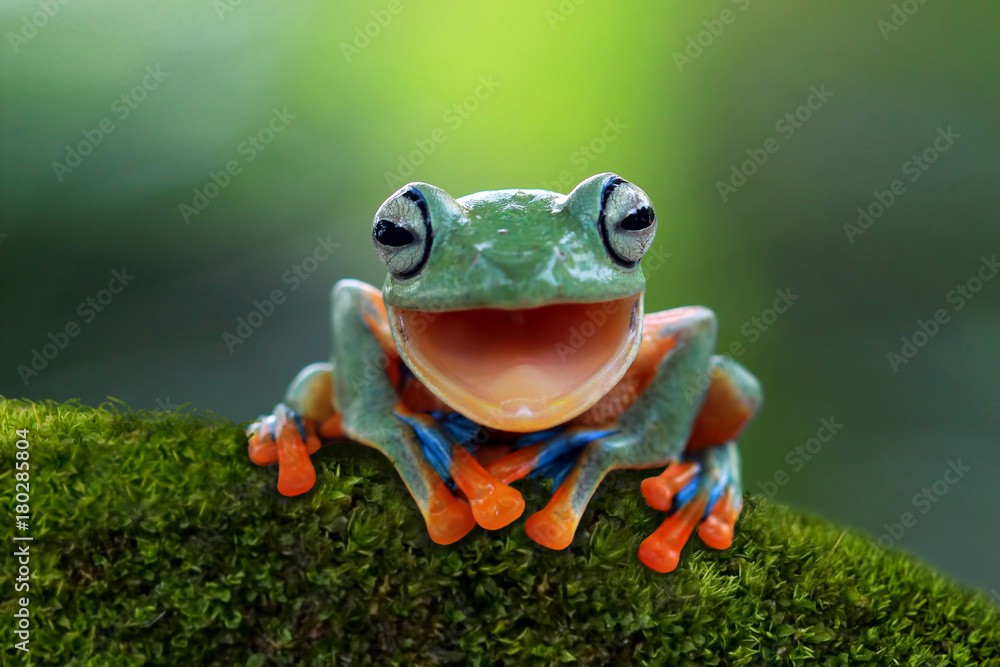
\includegraphics[scale=0.2]{frog}
	\end{wrapfigure}
	  }
\cfoot{ \footnotesize
Veškerý obsah najdete na webových stránkách gevotimes.gevo.cz \\
Na Facebooku jsme jako The GEVO Times a na Instagramu jako @gevotimes \\
Grafika a rozvržení: Eric Dusart
}
\rfoot{\footnotesize

}
\renewcommand{\headrulewidth}{0pt}
\renewcommand{\footrulewidth}{0.4pt}	% bar on bottom of page

\begin{document}

\sffamily
%Lines
\noindent
{\color{gray} \rule{\linewidth}{1pt}} \\[-0.5\baselineskip]
\noindent
{\color{black} \rule{\linewidth}{3pt}} \\[-0.65\baselineskip]
\noindent
{\color{gray} \rule{\linewidth}{1pt}}
 
\begin{multicols}{2}
	\setlength{\columnseprule}{1pt}
	

{\LARGE \textbf{Okénko třetích jazyků}}\\

V tomto novém segmentu TGT se podíváme na  nedávnou akci ve světě třetích jazyků. (A ne  nejsou to výstupky) Jedná se o španělskou  olympiádu ve které jsme jako škola měli velmi  silné zastoupení. Standardně se pořádalo více  kol na jiných úrovních. My jsme dostali tu  možnost vyzpovídat výtěžku jednoho z nich a  také naší studentku Báru Bytnarovou.\\

{\Large \textbf{Jak jsi se o této soutěži dozvěděla?}}\\

Z ničeho nic za mnou přišla za mnou pani 
profesorka Dimmerová a zeptala se mě jestli to 
nechci zkusit. Tak jsem si řekla proč ne. Nic se 
tím nezkazí a možná se i něco dozvím.\\

{\Large \textbf{A dá se třeba říct, že ti to pomohlo do nadcházejících 
výstupek?}}\\

Vzhledem k tomu, že to bylo velmi podobně
koncipováno tak se dá říct, že ano. Byla tam ta 
poslouchací část, popis obrázku a gramatika. 
Jediné co bylo nové byla reakce na nějakou 
situaci. Obecně to bylo ovšem o hodně delší a 
složitější.\\

{\Large \textbf{Myslíš si, že bychom jen z hodin a malým 
samostudiem mohli dosáhnout na této olympiádě
dobrých výsledků?}}\\

Tak já osobně mám ve škole ještě hodiny navíc s 
rodilým mluvčím kde se právě zaměřujeme na 
mluvení. Ale nemyslím si, že s naší školní výukou 
by studenti byli schopni uspět. Je to hlavně
dělané pro lidi které španělština baví takže dává 
smysl, že to není pro každého.\\

{\Large \textbf{Je někdo komu by jsi do příštích let doporučila účast 
na této olympiádě?}}\\

\begin{wrapfigure}{r}{0.15\textwidth}
	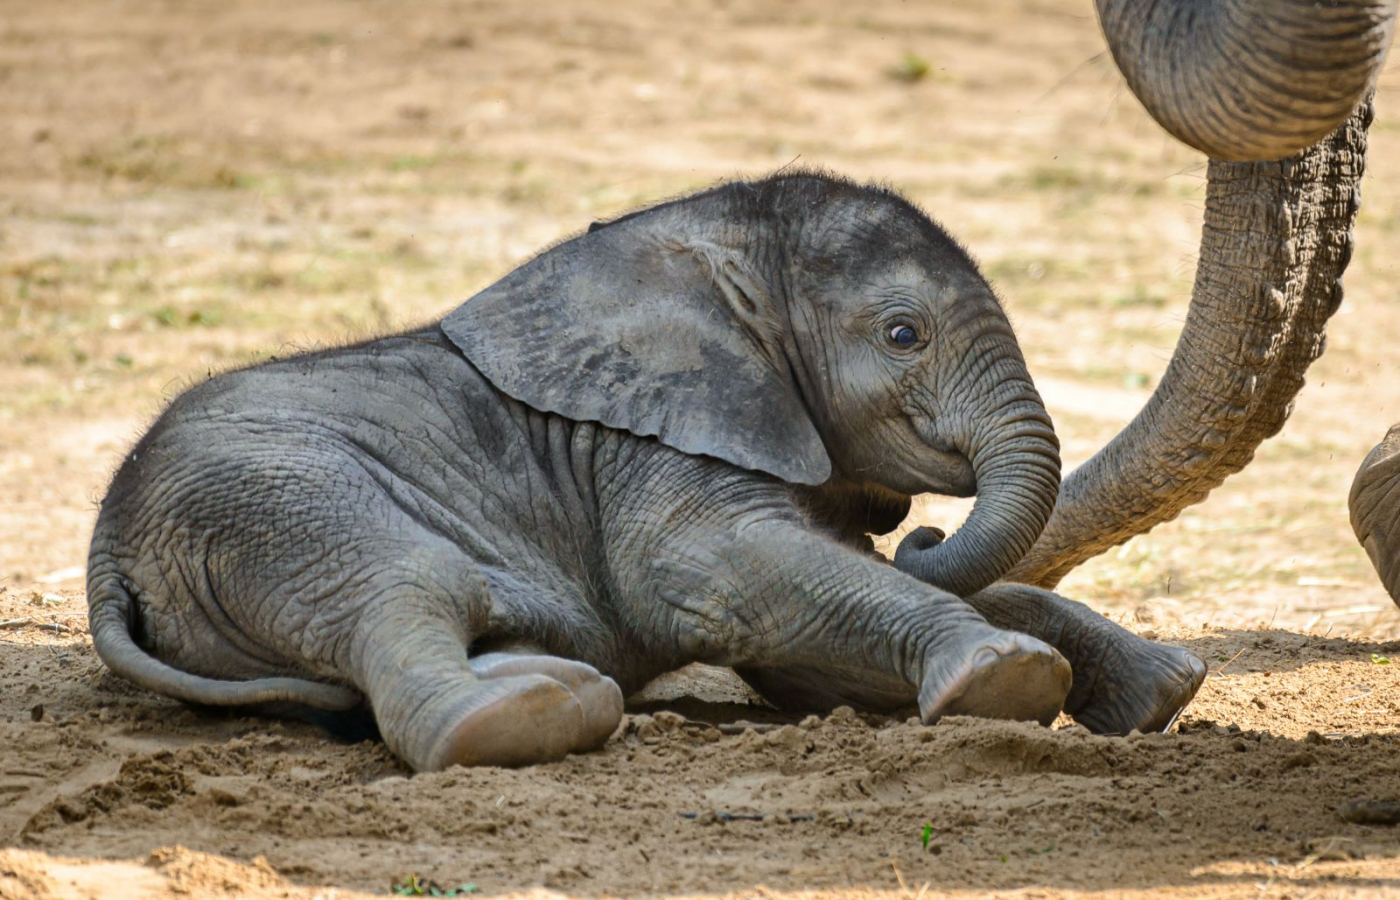
\includegraphics[width=1\linewidth]{elephant} 
\end{wrapfigure}
Tak jestli Vám nedělali výstupky problém a cítíte se trochu jistí se svojí španělštinou tak to rozhodně má smysl. Jediné na co je třeba si dávat pozor tak v druhém kole se objevovaly i otázky zaměřené. Třeba na geografii.

{\LARGE \textbf{Pozvánka na Terera}}\\

Drazí spolužáci, 
po roce se opět vrací tradiční školní anketa Zlatý
Terer. Pro ty z Vás, kteří by nevěděli co Zlatý
Terer je, přinášíme krátké shrnutí toho o co se 
jedná a jak akce funguje. Bla ha. qwekdj qwk edk q A pro ty z Vás, kteří už
vědí co a jak přinášíme informace k letošnímu 
ročníku. \\

Zlatý Terer je již tradiční akcí Gymnázia Evolution 
JM. Pořádána je vždy studenty předmaturitního 
ročníku (5. A/B a 3. C). Akce se pak tradičně pojí 
s celoškolní anketou, v rámci které studenti volí v 
mnoha kategoriích své favority. Mezi již tradiční 
soutěžní kategorie patří například Nejhezčí 
profesor/ka roku nebo Sportovec roku. 
Následuje přepočet hlasů, roznesení zlatých 
obálek s nominacemi a pak již hurá na slavnostní 
předávání cen! \\

Jak jste si tedy mohli přečíst, je na co se těšit. 
Kromě tradičního předávání cen Vás samozřejmě
čeká i mnohem více. Je dokonce v jednání 
možnost hudebního vystoupení v podání blíže 
nespecifikovaných profesorů. Dále se v minulých 
letech se objevila například i verze známé 
improvizační show Partička v podání učitelů. 
Nechme se tedy překvapit, co si pro nás letošní 
páťáci a třeťáci připravili. \\

Jak již tedy určitě všichni tušíte nebo víte, bude 
se na co těšit jako vždy. Popadněte tedy 
kamarády, sourozence nebo Vaše drahé 
polovičky a přijďte si užít s námi letošní ročník 
Zlatého Terera!!!\\

Těší se na Vás vaši páťáci a třeťáci!\\

Kdy? … 23.6.2022\\

Kde? To se brzy dozvíte na našem instagramu.\\

Lístky: v prodeji ve škole, spuštění prodeje se 
včas dozvíte\\

Dotazník: v emailových schránkách od 1.6.2022\\

Facebook: The GEVO Times\\

Instagram: terer 2022
\end{multicols}
\end{document}